\chapter{Tri par TAS}
\section {Description}
Il existe plusieurs types de méthodes de tri utilisées pour trier différents types de structures de données. L'une des méthodes de tri les plus populaires et les plus efficaces en informatique est le tri par tas.
\\
Le tri par tas  est une technique de tri basée sur la comparaison et basée sur la structure de données du tas.
\\
Tas (Heap en anglais) est une structure de données arborescente dans laquelle tous les nœuds de l'arbre sont dans un ordre spécifique. Tas est toujours un arbre binaire complet. 
\\
L'élément racine du Tas doit être à l'indice 0 dans le tableau.
\\
Pour le noeud à l'indice i :
\begin{itemize}
    \item  A l'indice (i-1)/2 se trouve le noeud parent.
    \item  A l'indice (2*i)+1, le nœud enfant gauche.
    \item  A l'index (2*i)+2, le noeud enfant de droite.
\end{itemize}


\section{Fonctionnement de l'algorithme}
L'algorithme du tri par tas fonctionne selon les étapes suivantes :
\begin{itemize}
 
     \item A partir des éléments du tableau donné, nous devons faire un tas maximum. Nous  commençons à empiler chaque sous-arbre de bas en haut et obtenir un max-heap après avoir appliqué la fonction à tous les éléments, y compris l'élément racine.
    \item  Retirer l'élément racine et le mettre à la fin du tableau (nième position) Mettre le dernier élément de l'arbre (tas) à la place vacante.
    \item  Réduire la taille du tas de 1.
    \item  Heapifier à nouveau l'élément racine de façon à avoir.
    \item l'élément le plus haut à la racine.
    \item Répétez ce processus encore et encore jusqu'à ce que tous les éléments de la liste soient triés dans le tableau avec succès.
\end{itemize}

\begin{figure}[H]
    \centering
        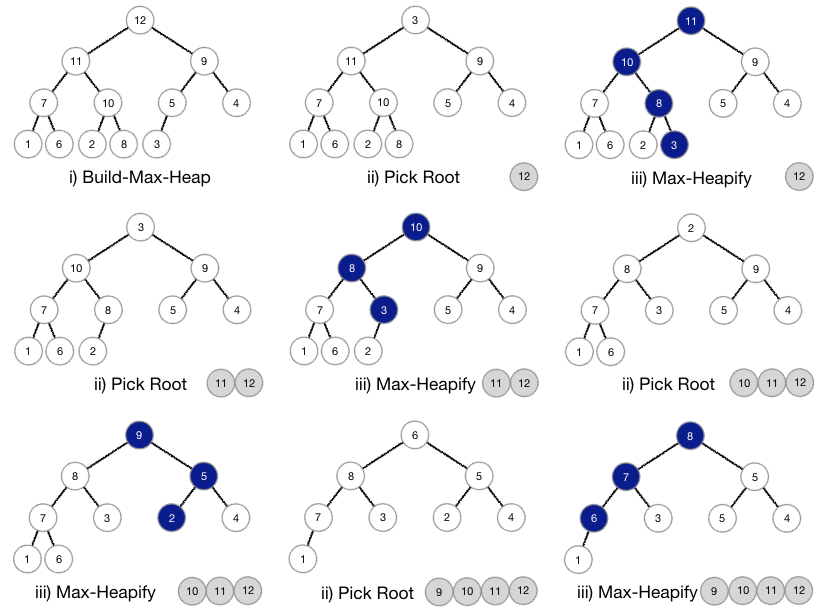
\includegraphics[scale=0.5]{ressources/HEAP.png}
        \caption{Exemple graphique d’un tri par tas}
    \label{fig:insert}
\end{figure}
Nous pouvons  représenter cet algorithme via le pseudo code suivant :
\par
\begin{function}[H]
    \textbf{Variables :}\\
    left,right : entier\;
    tmp,swapwith : entier\;
    
    
    \Begin{
        $left \leftarrow k*2-1 $\;
        $right \leftarrow k*2$\;
        $swapwith\leftarrow k-1 $\;
        \If{left<N et tab[left]>tab[swapwith]}
        {
               $swapwith\leftarrow left $\;
        }
        \If{right<N et tab[right]>tab[swapwith]}
        {
               $swapwith\leftarrow right $\;
        }
        \If{swapwith<>k-1}
        {
               $temp\leftarrow tab[swapwith] $\;
               $tab[swapwith]\leftarrow tab[k-1] $\;
               $tab[k-1] \leftarrow temp $\;
               heapify(tab,swapwith)\;
        }

      
    }
    \caption{heapify(Entrée: tab: tableau d'entier; k:entier;)}
\end{function}
\par
\begin{function}[H]
    \textbf{Variables :}\\
     temp,wn ,k: entier\;
    
    
    \Begin{
        \For{$k \leftarrow n/2$ \KwTo k>0}{
             heapify(tab,k)\; 
              $k\leftarrow k-1 $\;
         
            }
        \For{$wn \leftarrow n-1$ \KwTo wn>0}{
               $temp\leftarrow tab[0] $\;
               $tab[0]\leftarrow tab[wn] $\;
               $tab[wn] \leftarrow temp $\;
               heapify(tab,1)\;
            }
    }
    \caption{heapSort(Entrée: tab: tableau d'entier; )}
\end{function}
\section{Calcul de complexité}
\subsection{Complexité temporelle}
Heap Sort a des complexités temporelles O(nlog n) pour tous les cas (meilleur cas, cas moyen et pire cas).
\par
Dans la fonction heapify(), nous parcourons l'arbre de haut en bas. La hauteur d'un arbre binaire (la racine n'étant pas comptée) de taille n est log2 n au plus, c'est-à-dire que si le nombre d'éléments double, l'arbre ne devient plus profond que d'un niveau :
 \\
 \begin{figure}[H]
    \centering
        \includegraphics[scale=0.4]{ressources/complixité_tas.png}
        
    \label{fig:comtas}
\end{figure}

La complexité de la fonction heapify() est donc O(log n).
\\
\textbf{Complexité temporelle de la méthode HeapSort() :}

Pour construire initialement le tas, la méthode heapify () est appelée pour chaque nœud parent - en arrière, en commençant par le dernier nœud et en terminant à la racine de l'arbre.
\par
Un tas de taille n a n/2 nœuds parents (arrondis à l'inférieur) 
\par
La méthode heapify() est appelée n-1 fois. Ainsi, la complexité totale pour réparer le tas est également O(n log n).

\subsection{Complexité spatiale}
Étant donné que le tri en tas est un algorithme de tri conçu sur place, l'espace requis est constant, donc O (1). En effet, dans le cas de l'entrée :
\begin{enumerate}
  \item Nous utilisons la structure de tas pour organiser tous les éléments de la liste.
  \item Après avoir supprimé le plus grand nœud du tas max, nous plaçons l'élément supprimé à la fin de la même liste.
\end{enumerate}
Par conséquent, nous n'utilisons aucun espace supplémentaire lors de l'implémentation de cet algorithme. Cela donne à l'algorithme une complexité spatiale de O(1).
\\

\section{Experimentation}
Dans cette partie nous allons voir les résultats des exécutions de cet algorithme sur différents taille de tableau et sur données qui se représentent en 3 configuration ( triée en bon ordre , triée en ordre inverse , aléatoire) 
\subsubsection{Les données du tableau sont triées en bon ordre.}
\\
\begin{tabular}{| c | c | c | c | c | c | c | c | c | c | c |}
    \hline 
     Taille &  10000 & 50000 & 100000 & 500000 & 1000000 & 5000000 & 10000000 & 50000000 \\
    \hline
    temps(s) & 0,000066 &	0,000303	 & 0,000682	& 0,003029 & 0,00469 &	0,027033 & 0,062347 &	0,315974	 \\
   \hline
   
\end{tabular}
\par

\subsubsection{Les données du tableau sont triées en ordre inverse.}
\\
\begin{tabular}{| c | c | c | c | c | c | c | c | c | c | c |}
    \hline 
     Taille &  10000 & 50000 & 100000 & 500000 & 1000000 & 5000000 & 10000000 & 50000000 \\
    \hline
    temps(s) & 0,000052 &	0,00028 &	0,000643	 & 0,002413 &	0,005757 &	0,02379 &	0,049275 &	0,269919 \\
   
   \hline
\end{tabular}
\par
\subsubsection{Les données du tableau sont  positionnés aléatoirement.}
\\
\begin{tabular}{| c | c | c | c | c | c | c | c | c | c | c |}
    \hline 
     Taille &  10000 & 50000 & 100000 & 500000 & 1000000 & 5000000 & 10000000 & 50000000  \\
    \hline
    temps(s) & 0,000078 &	0,000384 &	0,000725	& 0,002596 &	0,004857 &	0,035832 &	0,057231 &	0,257452\\
    \hline
   
   
\end{tabular}
\par
\subsubsection{Le graphe :}
\\
La figure suivante représente les résultats d'exécution de cet algorithme selon les différentes taille du tableau.

\begin{figure}[H]
    \centering
        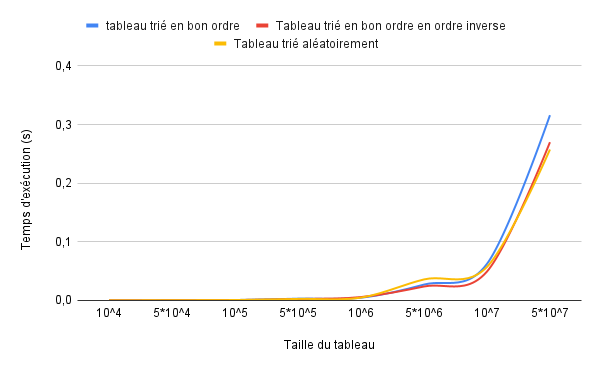
\includegraphics[scale=0.7]{ressources/heapchart.png}
        \caption{Temps d'execution du tri par tas sur les différents taille du tableau }
    \label{fig:insertch}
\end{figure}
\par
\par
D’après les graphes et les tableaux ci-dessus, Nous remarquons que le temps d’exécution évolue de manière quasi linéaire avec l’augmentation de la taille du tableau quel que soit sa configuration ( les 3 courbes sont presque  similaires) .
On en conclut que la complexité théorique est cohérente avec les résultats expérimentaux.

\section{Conclusion}
A partir d'étude expérimentale et théorique de l'algorithme tri par tas, On remarque que avec sa complexité temporelle de O(n log(n)) le tri en tas est toujours optimal. Il  a fonctionné avec succès sur les données  que nous avions prises et a obtenu des résultats satisfaisants pour les 3 configurations (table trié en ordre, table trié en inverse , table trié aleatoirement). 